  \subsubsection{Асимметричная схема дифракции}


  \begin{figure}[H]
    \centering
    \subfloat[$b = 33.52$, $\varphi$ > 0]{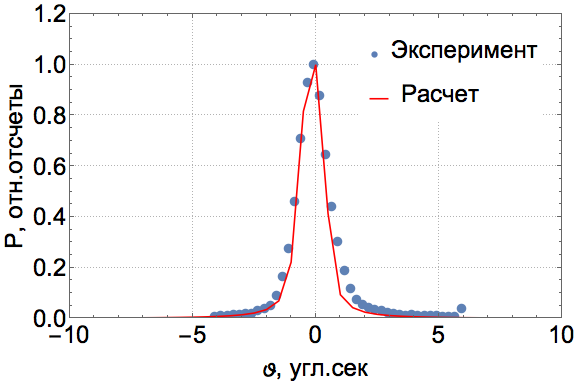
\includegraphics[width=0.45\textwidth]{images/assym-blue-50.png}}
    \hfill
    \subfloat[$b = 0.03$, $\varphi$ < 0]{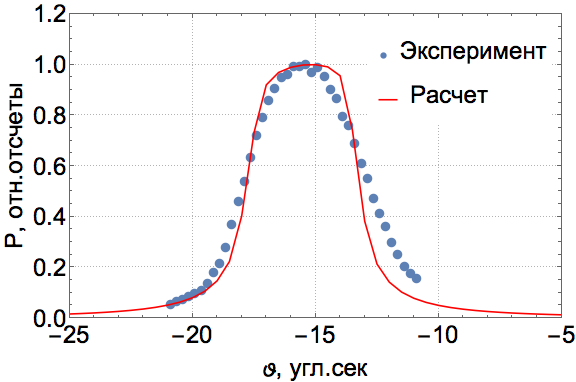
\includegraphics[width=0.45\textwidth]{images/assym-red-50.png}}
    \caption{Двухкристальная КДО для схемы с кристаллом монохроматором Si(440) и асимметричным образцом Si(440),
    угол разориентации поверхности $\varphi = 20^o53^{'}$. Размер щелевых устройств $S_1 = S_2 = 50$ мкм.}
    \label{ris:assymetric_exp_50}
  \end{figure}
